\documentclass[journal,12pt,twocolumn]{IEEEtran}

\usepackage{setspace}
\usepackage{gensymb}

\singlespacing


\usepackage[cmex10]{amsmath}

\usepackage{amsthm}

\usepackage{mathrsfs}
\usepackage{txfonts}
\usepackage{stfloats}
\usepackage{bm}
\usepackage{cite}
\usepackage{cases}
\usepackage{subfig}

\usepackage{longtable}
\usepackage{multirow}

\usepackage{enumitem}
\usepackage{mathtools}
\usepackage{steinmetz}
\usepackage{tikz}
\usepackage{circuitikz}
\usepackage{verbatim}
\usepackage{tfrupee}
\usepackage[breaklinks=true]{hyperref}
\usepackage{graphicx}
\usepackage{tkz-euclide}

\usetikzlibrary{calc,math}
\usepackage{listings}
\usepackage{color}                                            %%
\usepackage{array}                                            %%
\usepackage{longtable}                                        %%
\usepackage{calc}                                             %%
\usepackage{multirow}                                         %%
\usepackage{hhline}                                           %%
\usepackage{ifthen}                                           %%
\usepackage{lscape}     
\usepackage{multicol}
\usepackage{chngcntr}

\DeclareMathOperator*{\Res}{Res}

\renewcommand\thesection{\arabic{section}}
\renewcommand\thesubsection{\thesection.\arabic{subsection}}
\renewcommand\thesubsubsection{\thesubsection.\arabic{subsubsection}}

\renewcommand\thesectiondis{\arabic{section}}
\renewcommand\thesubsectiondis{\thesectiondis.\arabic{subsection}}
\renewcommand\thesubsubsectiondis{\thesubsectiondis.\arabic{subsubsection}}


\hyphenation{op-tical net-works semi-conduc-tor}
\def\inputGnumericTable{}                                 %%

\lstset{
	%language=C,
	frame=single, 
	breaklines=true,
	columns=fullflexible
}
\begin{document}
	
	
	\newtheorem{theorem}{Theorem}[section]
	\newtheorem{problem}{Problem}
	\newtheorem{proposition}{Proposition}[section]
	\newtheorem{lemma}{Lemma}[section]
	\newtheorem{corollary}[theorem]{Corollary}
	\newtheorem{example}{Example}[section]
	\newtheorem{definition}[problem]{Definition}
	
	\newcommand{\BEQA}{\begin{eqnarray}}
		\newcommand{\EEQA}{\end{eqnarray}}
	\newcommand{\define}{\stackrel{\triangle}{=}}
	\bibliographystyle{IEEEtran}
	\providecommand{\mbf}{\mathbf}
	\providecommand{\pr}[1]{\ensuremath{\Pr\left(#1\right)}}
	\providecommand{\qfunc}[1]{\ensuremath{Q\left(#1\right)}}
	\providecommand{\sbrak}[1]{\ensuremath{{}\left[#1\right]}}
	\providecommand{\lsbrak}[1]{\ensuremath{{}\left[#1\right.}}
	\providecommand{\rsbrak}[1]{\ensuremath{{}\left.#1\right]}}
	\providecommand{\brak}[1]{\ensuremath{\left(#1\right)}}
	\providecommand{\lbrak}[1]{\ensuremath{\left(#1\right.}}
	\providecommand{\rbrak}[1]{\ensuremath{\left.#1\right)}}
	\providecommand{\cbrak}[1]{\ensuremath{\left\{#1\right\}}}
	\providecommand{\lcbrak}[1]{\ensuremath{\left\{#1\right.}}
	\providecommand{\rcbrak}[1]{\ensuremath{\left.#1\right\}}}
	\theoremstyle{remark}
	\newtheorem{rem}{Remark}
	\newcommand{\sgn}{\mathop{\mathrm{sgn}}}
	\providecommand{\abs}[1]{\left\vert#1\right\vert}
	\providecommand{\res}[1]{\Res\displaylimits_{#1}} 
	\providecommand{\norm}[1]{\left\lVert#1\right\rVert}
	%\providecommand{\norm}[1]{\lVert#1\rVert}
	\providecommand{\mtx}[1]{\mathbf{#1}}
	\providecommand{\mean}[1]{E\left[ #1 \right]}
	\providecommand{\fourier}{\overset{\mathcal{F}}{ \rightleftharpoons}}
	%\providecommand{\hilbert}{\overset{\mathcal{H}}{ \rightleftharpoons}}
	\providecommand{\system}{\overset{\mathcal{H}}{ \longleftrightarrow}}
	%\newcommand{\solution}[2]{\textbf{Solution:}{#1}}
	\newcommand{\solution}{\noindent \textbf{Solution: }}
	\newcommand{\cosec}{\,\text{cosec}\,}
	\providecommand{\dec}[2]{\ensuremath{\overset{#1}{\underset{#2}{\gtrless}}}}
	\newcommand{\myvec}[1]{\ensuremath{\begin{pmatrix}#1\end{pmatrix}}}
	\newcommand{\mydet}[1]{\ensuremath{\begin{vmatrix}#1\end{vmatrix}}}
	\numberwithin{equation}{subsection}
	\makeatletter
	\@addtoreset{figure}{problem}
	\makeatother
	\let\StandardTheFigure\thefigure
	\let\vec\mathbf
	\renewcommand{\thefigure}{\theproblem}
	\def\putbox#1#2#3{\makebox[0in][l]{\makebox[#1][l]{}\raisebox{\baselineskip}[0in][0in]{\raisebox{#2}[0in][0in]{#3}}}}
	\def\rightbox#1{\makebox[0in][r]{#1}}
	\def\centbox#1{\makebox[0in]{#1}}
	\def\topbox#1{\raisebox{-\baselineskip}[0in][0in]{#1}}
	\def\midbox#1{\raisebox{-0.5\baselineskip}[0in][0in]{#1}}
	\vspace{3cm}
	
	
	
	\title{EE5609 Assignment 5}
	\author{Vimal K B \\Roll No - AI20MTECH14002}
	
	\maketitle
	\newpage
	%\tableofcontents
	\bigskip
	
	\renewcommand{\thefigure}{\theenumi}
	\renewcommand{\thetable}{\theenumi}
	
	\begin{abstract}
		This assignment involves proving the equivalence of 2 lines that are formed inside an isosceles triangle because of certain given conditions via vector representation.
	\end{abstract}

	Download all latex-tikz codes from 
	
	\begin{lstlisting}
		https://github.com/vimalkb007/EE5609/tree/master/Assignment_5
	\end{lstlisting}
	
	\section{Problem Statement}
In an isosceles $\triangle ABC$ with $AB$ = $AC$, D and E are points on $BC$ such that $BE = CD$. Show that $AD = AE$. 
	\section{Solution}
	
	In the given  $\triangle ABC$, let $D$ and $E$ be any arbitrary points on the side $BC$ such that $\vec{BE}$ = $\vec{CD}$.
	
	\renewcommand{\thefigure}{1}
	\begin{figure}[!ht] \label{fig:two_triangles}
		\centering
		\resizebox{\columnwidth}{!}{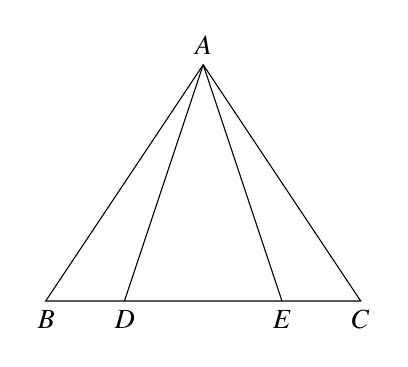
\begin{tikzpicture} 
%	\coordinate (A) at (2, 3) {};
%	\coordinate (B) at (0, 0) {};
%	\coordinate (C) at (4, 0) {};
%	\coordinate (D) at (1, 0) {};
%	\coordinate (E) at (3, 0) {};
%	\draw (A)node[above]{$A$}--(B)node[below]{$B$}--(C)node[below]{$C$}--cycle;
%	\draw (B)node[below]{}--(E)node[below]{$E$};
%	\draw (C)node[below]{}--(D)node[below]{$D$};
	
	
	
	\coordinate (A) at (2,3){};
	\coordinate (B) at (0, 0){};
	\coordinate (C) at (4, 0){};
	\coordinate (D) at (1, 0){};
	\coordinate (E) at (3, 0){};
	
	%Drawing triangle ABC
	\draw (A)node[above]{$A$}--(B)node[below]{$B$}--(C)node[below]{$C$}--cycle;
	\draw (A)node[above]{}--(D)node[below]{$D$};
	\draw (A)node[above]{}--(E)node[below]{$E$};
	
\end{tikzpicture}}
		\caption{Isosceles Triangle with sides AB = AC}
	\end{figure}
	We are given that the sides $AB = AC$, and $BE = CD$. These two can be represented as
	\begin{align}\label{eq:fact1}
		\norm{B-A} = \norm{C-A}
	\end{align}
	\begin{align}\label{eq:fact2}
		\norm{B-E} = \norm{D-C}
	\end{align}
	
	Since the given trianle is an isoceles triangle, the angles formed by $AB$ and $AC$ on $BC$ will be the same. That is
	\begin{align}\label{eq:fact3}
		\angle ABC = \angle ACB = \alpha
	\end{align}
	The side $AD$ can be represented as 
	\begin{align}\label{eq:eq1}
		(\vec{D-A}) = (\vec{B-A}) - (\vec{B-D})
	\end{align}
	Squaring both the sides we get	
	\begin{align} \label{eq:eq2}
		\norm{D-A}^{2} = \norm{B-A}^{2} + \norm{B-D}^{2} - 2\norm{B-A}\norm{B-D}\cos\alpha
	\end{align}
	The side $AE$ can be represented as 
	\begin{align}\label{eq:eq3}
		(\vec{A-E}) = (\vec{C-A}) - (\vec{C-E})
	\end{align}
	Squaring both the sides we get	
	\begin{align} \label{eq:eq4}
		\norm{A-E}^{2} = \norm{C-A}^{2} + \norm{C-E}^{2} - 2\norm{C-A}\norm{C-E}\cos\alpha
	\end{align}
	
	From \eqref{eq:fact2}, we can further write it as 
	\begin{align}\label{eq:eq5}
		\norm{E-B}) = \norm{B-D} + \norm{E-D}
	\end{align}
	\begin{align}\label{eq:eq6}
		\norm{C-D} = \norm{C-E} + \norm{E-D}
	\end{align}
	From equations \eqref{eq:fact2}, \eqref{eq:eq5} and \eqref{eq:eq6} we can equate the L.H.S and get
	
	\begin{align}\label{eq:eq7}
		\norm{B-D} = \norm{C-E}
	\end{align}

	Using equations \eqref{eq:fact1}, \eqref{eq:eq7}, we apply them in the equation \eqref{eq:eq2}, \eqref{eq:eq4}. After applying it we see that the R.H.S components are getting equated to each other, then we can equate the L.H.S as well. We get 
	\begin{align}\label{eq:eq8}
		\norm{D-A}^{2} = \norm{A-E}^{2} \nonumber \\
		\norm{D-A} = \norm{A-E}
	\end{align}
	
	Therefore, we can say that $AD = AE$.
	
\end{document}